\documentclass{article}
\usepackage[utf8]{inputenc}
\usepackage[margin=1.0in]{geometry}
\usepackage[section]{placeins}
\usepackage{graphicx}
\graphicspath{ {./images/} }
\begin{document}

\section*{NYT Phrase Rank Lists}
From left to right, below is the list of top 30, middle 30, and bottom 30 single word phrases for the NYT dataset with the suggested parameters of $HIGHLIGHT\_SINGLE=.9$ and $HIGHLIGHT\_MULTI=.5$.\\
\begin{table}[ht]
\parbox{.22\linewidth}{
\centering
\begin{tabular}{|c|c|}
\hline
wbc & 0.8512157704 \\
\hline
minneapolis & 0.8472041311 \\
\hline
dna & 0.8470183261 \\
\hline
cska & 0.8468338448 \\
\hline
cbs & 0.8423605647 \\
\hline
wellington & 0.8421586470 \\
\hline
iv & 0.8421261359 \\
\hline
fbi & 0.8420124957 \\
\hline
dc & 0.8414233784 \\
\hline
nba & 0.8411841758 \\
\hline
fx & 0.8405590938 \\
\hline
istanbul & 0.8399355593 \\
\hline
prague & 0.8398781518 \\
\hline
amc & 0.8394182441 \\
\hline
rbs & 0.8389925043 \\
\hline
clarence & 0.8389280748 \\
\hline
lima & 0.8385657743 \\
\hline
sacramento & 0.8385282580 \\
\hline
tripoli & 0.8381023545 \\
\hline
dublin & 0.8379963028 \\
\hline
lgbt & 0.8379090817 \\
\hline
bcs & 0.8374214900 \\
\hline
usa & 0.8372757945 \\
\hline
albany & 0.8370727411 \\
\hline
naples & 0.8368999479 \\
\hline
lexington & 0.8368385291 \\
\hline
cal & 0.8363055371 \\
\hline
milan & 0.8362579035 \\
\hline
amsterdam & 0.8361695801 \\
\hline
\end{tabular}
\caption{Top 30}
}
\hfill
\parbox{.22\linewidth}{
\centering
\begin{tabular}{|c|c|}
\hline
intentional & 0.5870088101 \\
\hline
prodded & 0.5870083729 \\
\hline
ordinarily & 0.5870083729 \\
\hline
confront & 0.5870008670 \\
\hline
soprano & 0.5869853623 \\
\hline
machinery & 0.5869702128 \\
\hline
riot & 0.5869621683 \\
\hline
waiting & 0.5869557429 \\
\hline
atrocities & 0.5869556507 \\
\hline
prevail & 0.5869546957 \\
\hline
here’s & 0.5869530878 \\
\hline
interrupted & 0.5869266819 \\
\hline
smokers & 0.5869212730 \\
\hline
disruption & 0.5868902329 \\
\hline
originally & 0.5868889273 \\
\hline
slam & 0.5868875053 \\
\hline
poisoning & 0.5868756404 \\
\hline
desperately & 0.5868640156 \\
\hline
siege & 0.5868636363 \\
\hline
widow & 0.5868611921 \\
\hline
buy & 0.5868535537 \\
\hline
recreational & 0.5868499478 \\
\hline
hosting & 0.5868189940 \\
\hline
unusually & 0.5867760126 \\
\hline
wheelchairs & 0.5867586481 \\
\hline
torque & 0.5867586481 \\
\hline
strikes & 0.5867349929 \\
\hline
ribs & 0.5867307076 \\
\hline
endless & 0.5867247648 \\
\hline
\end{tabular}
\caption{Mid 30}
}
\hfill
\parbox{.23\linewidth}{
\centering
\begin{tabular}{|c|c|}
\hline
172 & 0.2744979322 \\
\hline
06 & 0.2742260498 \\
\hline
332 & 0.2739979322 \\
\hline
299 & 0.2739979322 \\
\hline
285 & 0.2739979322 \\
\hline
139 & 0.2738766169 \\
\hline
126 & 0.2734599502 \\
\hline
214 & 0.2734599502 \\
\hline
03 & 0.2728980737 \\
\hline
320 & 0.2728980737 \\
\hline
325 & 0.2726260498 \\
\hline
157 & 0.2724599502 \\
\hline
02 & 0.2723790519 \\
\hline
375 & 0.2723790519 \\
\hline
containing & 0.2721296301 \\
\hline
158 & 0.2719718549 \\
\hline
380 & 0.2719718549 \\
\hline
116 & 0.2710698596 \\
\hline
specified & 0.2696099502 \\
\hline
124 & 0.2694850748 \\
\hline
145 & 0.2691612652 \\
\hline
280 & 0.2685555739 \\
\hline
107 & 0.2683433052 \\
\hline
111 & 0.2678667286 \\
\hline
112 & 0.2673443406 \\
\hline
114 & 0.2667911009 \\
\hline
sincere & 0.2666137439 \\
\hline
ought & 0.2653443406 \\
\hline
102 & 0.2644190375 \\
\hline
\end{tabular}
\caption{Bottom 30}
}
\end{table}\\
These lists above make sense because the top 30 are all common acronyms and proper nouns, the mid 30 are frequent and meaningful nouns and verbs, and the bottom 30 are mostly random numbers.\\\\\\
From left to right, below is the list of top 30, middle 30, and bottom 30 multi word phrases for the NYT dataset with the suggested parameters of $HIGHLIGHT\_SINGLE=.9$ and $HIGHLIGHT\_MULTI=.5$.\\
These lists below for multi word phrases are intuitive because the top 30 are names of people and organizations, the middle 30 are common phrases in speech, and the bottom 30 are prepositions and transitional phrases.
\begin{table}[ht]
\parbox{.16\linewidth}{
\centering
\begin{tabular}{|c|c|}
\hline
kyrie irving & 0.9859670300\\
\hline
adrian peterson & 0.9858567268\\
\hline
justin bieber & 0.9855607233\\
\hline
aston villa & 0.9852497353\\
\hline
richie incognito & 0.9851547916\\
\hline
marshawn lynch & 0.9848564661\\
\hline
fidel castro & 0.9845802860\\
\hline
napa valley & 0.9845547987\\
\hline
graeme swann & 0.9843076584\\
\hline
nick saban & 0.9842913079\\
\hline
rafael nadal & 0.9841839528\\
\hline
henrik lundqvist & 0.9841120842\\
\hline
justin timberlake & 0.9840859622\\
\hline
gareth bale & 0.9840295465\\
\hline
tiger woods & 0.9839738113\\
\hline
jamaal charles & 0.9839603943\\
\hline
sears holdings & 0.9839533040\\
\hline
dwight howard & 0.9838893572\\
\hline
alan mulally & 0.9838876767\\
\hline
derek stepan & 0.9838231328\\
\hline
walt disney & 0.9837392413\\
\hline
nick foles & 0.9836625843\\
\hline
michel djotodia & 0.9836394567\\
\hline
brook lopez & 0.9835856279\\
\hline
hurricane katrina & 0.9835716916\\
\hline
tim duncan & 0.9835537588\\
\hline
ubs ag & 0.9835314120\\
\hline
sebastian vettel & 0.9834178661\\
\hline
janet yellen & 0.9833784342\\
\hline
golan heights & 0.9833098495\\
\hline
\end{tabular}
\caption{Top 30}
}
\hfill
\parbox{.22\linewidth}{
\centering
\begin{tabular}{|c|c|}
\hline
handed down & 0.1278334721\\
\hline
stand up & 0.1278236174\\
\hline
ranges from & 0.1278187086\\
\hline
from public life & 0.1278089004\\
\hline
of comcast corp & 0.1277916275\\
\hline
wars in iraq and & 0.1277562480\\
\hline
doesn't include & 0.1277504663\\
\hline
energy bill & 0.1277337884\\
\hline
as south africa's & 0.1277202886\\
\hline
well aware & 0.1277180673\\
\hline
35 minutes & 0.1277144797\\
\hline
in tax breaks & 0.1277116959\\
\hline
israeli military said & 0.1276519684\\
\hline
get hurt & 0.1276420641\\
\hline
gave me & 0.1276355675\\
\hline
of political prisoners & 0.1276305578\\
\hline
announced tuesday that & 0.1275690246\\
\hline
in june 2012 & 0.1275658157\\
\hline
dominican republic and & 0.1275312384\\
\hline
slightly better & 0.1275279922\\
\hline
political system & 0.1275074171\\
\hline
to enlist & 0.1275043352\\
\hline
left behind & 0.1274784624\\
\hline
last four years & 0.1274718913\\
\hline
still alive & 0.1274561571\\
\hline
without power & 0.1274171262\\
\hline
reunite with & 0.1273897374\\
\hline
former employees & 0.1273891631\\
\hline
to be & 0.1273639799\\
\hline
60 years & 0.1273436734\\
\hline
\end{tabular}
\caption{Mid 30}
}
\hfill
\parbox{.23\linewidth}{
\centering
\begin{tabular}{|c|c|}
\hline
one hand and & 0.0075959662\\
\hline
of months of & 0.0075959662\\
\hline
of pennsylvania and & 0.0075959662\\
\hline
to syria to & 0.0075959662\\
\hline
from home and & 0.0075959662\\
\hline
three games with & 0.0075959662\\
\hline
of meetings with & 0.0075959662\\
\hline
for consumers to & 0.0075959662\\
\hline
a lot to & 0.0075959662\\
\hline
to happen in & 0.0075959662\\
\hline
of murder in & 0.0075959662\\
\hline
in court on & 0.0075959662\\
\hline
for oil and & 0.0075959662\\
\hline
nine years in & 0.0075959662\\
\hline
to sign with & 0.0075959662\\
\hline
to grant a & 0.0075959662\\
\hline
to file for & 0.0075959662\\
\hline
to die in & 0.0075959662\\
\hline
in mind that & 0.0075959662\\
\hline
of violence in the & 0.0075959662\\
\hline
of millions of people & 0.0075959662\\
\hline
for sale in & 0.0075959662\\
\hline
to study in & 0.0075959662\\
\hline
to turn this & 0.0075959662\\
\hline
in court that & 0.0075959662\\
\hline
of billions of & 0.0075959662\\
\hline
to reporters at & 0.0075959662\\
\hline
of money in & 0.0075959662\\
\hline
of state for & 0.0075959662\\
\hline
said she & 0.0070537286\\
\hline
\end{tabular}
\caption{Bottom 30}
}
\end{table}
\section*{Yelp Phrase Rank Lists}
From left to right, the lists on the following page are of the top 30, middle 30, and bottom 30 single word phrases for the NYT dataset with the suggested parameters of $HIGHLIGHT\_SINGLE=.9$ and $HIGHLIGHT\_MULTI=.5$.\\
These lists make sense because the top 30 are mostly all names of foods and drinks, the middle 30 are common nouns and verbs associated with restaurants and services, and the bottom 30 are mostly prepositions that don't have much meaning.\\\\
The lists on page 4 are the top, middle and bottom 30 multi word phrases in the Yelp dataset.  Again these lists are intuitive because the top 30 are organization names or names of specific foods, the middle 30 are common foods and speech phrases, and the bottom 30 are more prepositions and transitions.
\begin{table}[ht]
\parbox{.22\linewidth}{
\centering
\begin{tabular}{|c|c|}
\hline
trail & 0.9283774739 \\
\hline
ale & 0.9279517675 \\
\hline
sangria & 0.9251320512 \\
\hline
yelper & 0.9231119693 \\
\hline
hangover & 0.9215918356 \\
\hline
eggplant & 0.9210159397 \\
\hline
gold & 0.9208643534 \\
\hline
library & 0.9205310201 \\
\hline
stew & 0.9190822358 \\
\hline
church & 0.9189934626 \\
\hline
latte & 0.9187752054 \\
\hline
cherry & 0.9184212028 \\
\hline
espresso & 0.9181488972 \\
\hline
yelpers & 0.9176200685 \\
\hline
vegas & 0.9171503716 \\
\hline
viet & 0.9168684378 \\
\hline
brie & 0.9168375948 \\
\hline
mole & 0.9162541174 \\
\hline
lifetime & 0.9160440823 \\
\hline
flatbread & 0.9158635588 \\
\hline
parmesan & 0.9155271740 \\
\hline
brewery & 0.9152714963 \\
\hline
ribeye & 0.9152654524 \\
\hline
zin & 0.9152449625 \\
\hline
meatball & 0.9151991072 \\
\hline
fitness & 0.9151448717 \\
\hline
farms & 0.9150685900 \\
\hline
coach & 0.9150399127 \\
\hline
ranch & 0.9150369352 \\
\hline
\end{tabular}
\caption{Top 30}
}
\hfill
\parbox{.24\linewidth}{
\centering
\begin{tabular}{|c|c|}
\hline
kinda & 0.7716520296 \\
\hline
basement & 0.7716468228 \\
\hline
fricken & 0.7716241467 \\
\hline
posts & 0.7716208485 \\
\hline
caliber & 0.7716175362 \\
\hline
diverse & 0.7716133299 \\
\hline
dimsum & 0.7716003917 \\
\hline
famed & 0.7715747751 \\
\hline
cheezy & 0.7715329133 \\
\hline
preschool & 0.7715329133 \\
\hline
isolated & 0.7715109722 \\
\hline
hope & 0.7714825538 \\
\hline
traditionally & 0.7714700443 \\
\hline
haircut & 0.7714621814 \\
\hline
lengthy & 0.7714562774 \\
\hline
attendance & 0.7714516128 \\
\hline
resteraunt & 0.7714475621 \\
\hline
pigeons & 0.7714475621 \\
\hline
app's & 0.7714475621 \\
\hline
ashes & 0.7714475621 \\
\hline
leadership & 0.7714475621 \\
\hline
issue & 0.7714269907 \\
\hline
43rd & 0.7714168844 \\
\hline
ubiquitous & 0.7713882299 \\
\hline
softener & 0.7713855170 \\
\hline
chipper & 0.7713338390 \\
\hline
wage & 0.7713290252 \\
\hline
sites & 0.7713123338 \\
\hline
days & 0.7713087739 \\
\hline
\end{tabular}
\caption{Mid 30}
}
\hfill
\parbox{.21\linewidth}{
\centering
\begin{tabular}{|c|c|}
\hline
amongst & 0.3745894890 \\
\hline
06 & 0.3734362821 \\
\hline
werent & 0.3732478184 \\
\hline
been & 0.3732182178 \\
\hline
which & 0.3727403290 \\
\hline
containing & 0.3723831115 \\
\hline
09 & 0.3723831115 \\
\hline
yourself & 0.3710446346 \\
\hline
me & 0.3708902248 \\
\hline
awfully & 0.3707345023 \\
\hline
02 & 0.3707345023 \\
\hline
becomes & 0.3707275842 \\
\hline
can & 0.3704885490 \\
\hline
merely & 0.3704784044 \\
\hline
could & 0.3700245072 \\
\hline
05 & 0.3674529488 \\
\hline
be & 0.3664271359 \\
\hline
gives & 0.3662908717 \\
\hline
themselves & 0.3659551358 \\
\hline
him & 0.3632958684 \\
\hline
have & 0.3631863165 \\
\hline
ourselves & 0.3618827637 \\
\hline
is & 0.3612317711 \\
\hline
has & 0.3610493581 \\
\hline
them & 0.3608067799 \\
\hline
are & 0.3587614793 \\
\hline
were & 0.3577612489 \\
\hline
was & 0.3570231537 \\
\hline
myself & 0.3561846821 \\
\hline
\end{tabular}
\caption{Bottom 30}
}
\end{table}\\\\
\begin{table}[ht]
\parbox{.18\linewidth}{
\centering
\begin{tabular}{|c|c|}
\hline
jamba juice & 0.9855316025\\
\hline
grand marnier & 0.9837130519\\
\hline
hyatt regency & 0.9834038475\\
\hline
botanical gardens & 0.9819158655\\
\hline
jimmy johns & 0.9815106738\\
\hline
hobby lobby & 0.9798741782\\
\hline
palo verde & 0.9795939574\\
\hline
del rey & 0.9795771212\\
\hline
orange blossom & 0.9792773294\\
\hline
peter piper & 0.9791724839\\
\hline
taliesin west & 0.9789654644\\
\hline
cheesecake factory & 0.9788442154\\
\hline
cabernet sauvignon & 0.9786717397\\
\hline
del mar & 0.9785584259\\
\hline
english muffin & 0.9782791894\\
\hline
chile relleno & 0.9782021344\\
\hline
el paso & 0.9781792604\\
\hline
pollo asado & 0.9781085274\\
\hline
daily dose & 0.9780325640\\
\hline
red robin & 0.9780062009\\
\hline
squaw peak & 0.9779615017\\
\hline
union hills & 0.9779233649\\
\hline
upper crust & 0.9777963502\\
\hline
delhi palace & 0.9777607192\\
\hline
carl's jr & 0.9777348202\\
\hline
johnny rockets & 0.9776970828\\
\hline
tater tots & 0.9776615624\\
\hline
michael mina & 0.9776529286\\
\hline
ann taylor & 0.9776391505\\
\hline
dos equis & 0.9775953971\\
\hline
\end{tabular}
\caption{Top 30}
}
\hfill
\parbox{.24\linewidth}{
\centering
\begin{tabular}{|c|c|}
\hline
the wedge salad & 0.0885694854\\
\hline
sitting on top of & 0.0885663980\\
\hline
the old days & 0.0885654616\\
\hline
a bad choice & 0.0885610444\\
\hline
bent on & 0.0885559050\\
\hline
especially since & 0.0885509178\\
\hline
a shopping center & 0.0885478251\\
\hline
the mediterranean & 0.0885436086\\
\hline
with arugula & 0.0885353958\\
\hline
flow of & 0.0885310512\\
\hline
an incredible & 0.0885294980\\
\hline
that point & 0.0885292634\\
\hline
driving into & 0.0885289634\\
\hline
the easiest & 0.0885265352\\
\hline
starting to get & 0.0885263643\\
\hline
particularly care for & 0.0885217908\\
\hline
to order drinks & 0.0885201542\\
\hline
to dance & 0.0885161429\\
\hline
by weight & 0.0885105557\\
\hline
a medium & 0.0885099993\\
\hline
diagnosed with & 0.0885098387\\
\hline
away from & 0.0885085989\\
\hline
at ikea & 0.0885037011\\
\hline
a nice outdoor patio & 0.0884998262\\
\hline
does not matter & 0.0884994810\\
\hline
all night & 0.0884984343\\
\hline
for sunday brunch & 0.0884845028\\
\hline
a yummy & 0.0884817247\\
\hline
every other & 0.0884773489\\
\hline
an enthusiastic & 0.0884728286\\
\hline
\end{tabular}
\caption{Mid 30}
}
\hfill
\parbox{.24\linewidth}{
\centering
\begin{tabular}{|c|c|}
\hline
to venture to & 0.0067325702\\
\hline
a search for & 0.0067175661\\
\hline
to go again and & 0.0066756286\\
\hline
some research on & 0.0065839591\\
\hline
got seated at & 0.0065818086\\
\hline
no issues with & 0.0065001504\\
\hline
and it's fun to & 0.0064707003\\
\hline
1 star because & 0.0064616889\\
\hline
and just wanted to & 0.0064463948\\
\hline
the nail on & 0.0064420109\\
\hline
and can't wait to go & 0.0064151448\\
\hline
and very easy to & 0.0063960832\\
\hline
people complain about & 0.0063864553\\
\hline
i'm working on & 0.0061836335\\
\hline
usually sit at & 0.0061836335\\
\hline
got tired of & 0.0061514703\\
\hline
actually care about & 0.0061280780\\
\hline
very reminiscent of & 0.0061191174\\
\hline
so i'll keep & 0.0061012530\\
\hline
the peak of & 0.0060635619\\
\hline
i've worked in & 0.0059302285\\
\hline
a touch more & 0.0059302285\\
\hline
to relax with & 0.0059064550\\
\hline
a block of & 0.0058506258\\
\hline
to call ahead and & 0.0058439550\\
\hline
to kick back & 0.0057881258\\
\hline
the only drawback to & 0.0057675661\\
\hline
a cheeseburger with & 0.0057606217\\
\hline
a scale of & 0.0057047924\\
\hline
any combination of & 0.0049302285\\
\hline
\end{tabular}
\caption{Bottom 30}
}
\end{table}\\
\section*{Phrasal Segmentation Metrics}
The below table shows the number of unique qualified phrases and average number of phrases per sentence for each dataset for $HIGHLIGHT\_SINGLE=.9$ and $HIGHLIGHT\_MULTI=.5$.  These metrics include both single and multi word phrases.
\begin{table}[ht]
    \centering
    \begin{tabular}{|c|c|c|}
        \hline
        & NYT & Yelp \\
        \hline
        Avg per sentence & .94149 & .780041 \\
        \hline
        Total unique phrases & 65552 & 41988\\
        \hline
    \end{tabular}
    \caption{Phrase metrics}
    \label{tab:my_label}
\end{table}\\
Since NYT is professionally written and edited, I would expect a natural language processor to more easily identify phrases, which is reflected in the data.  Yelp reviews contain a lot of slang and bad grammar, which might make the task of identifying phrases more difficult, yielding fewer phrases identified overall.\\\\
\section*{NYT Phrase Clusters}
Below are samples of six clusters obtained from using the k means algorithm with 75 centers on the NYT dataset.  I only clustered phrases returned by AutoPhrase and used each phrase's vector from word2vec to do the clustering.  I've labeled the concept each cluster is describing in the table captions.
\begin{table}[ht]
    \parbox{.3\linewidth}{
    \centering
    \begin{tabular}{|c|}
    \hline
    \_government\_\\
    \hline
    \_state\_\\
    \hline
    \_country\_\\
    \hline
    \_public\_\\
    \hline
    \_city\_\\
    \hline
    \_capital\_\\
    \hline
    \_Syria\_\\
    \hline
    \_corruption\_\\
    \hline
    \_politics\_\\
    \hline
    \_army\_\\
    \hline
    \_Iraq\_\\
    \hline
    \_Muslim\_\\
    \hline
    \_Islamic\_\\
    \hline
    \_Islamist\_\\
    \hline
    \_wave\_\\
    \hline
    \_Assad\_\\
    \hline
    \_ethnic\_\\
    \hline
    \_suicide\_\\
    \hline
    \_Libya\_\\
    \hline
    \_toll\_\\
    \hline
    \end{tabular}
    \caption{Middle East Politics}
    }
    \hfill
    \parbox{.24\linewidth}{
    \centering
    \begin{tabular}{|c|}
    \hline
    \_revenue\_\\
    \hline
    \_range\_\\
    \hline
    \_auction\_\\
    \hline
    \_billion\_euros\_\\
    \hline
    \_million\_euros\_\\
    \hline
    \_million\_pounds\_\\
    \hline
    \_euros\_\\
    \hline
    \_acres\_\\
    \hline
    \_billion\_pounds\_\\
    \hline
    \_lease\_\\
    \hline
    \_temperature\_\\
    \hline
    \_square\_feet\_\\
    \hline
    \_ticket\_sales\_\\
    \hline
    \_trillion\_yen\_\\
    \hline
    \_miles\_per\_hour\_\\
    \hline
    \_million\_shares\_\\
    \hline
    \_contemporary\_art\_\\
    \hline
    \_square\_foot\_\\
    \hline
    \_million\_Americans\_\\
    \hline
    \_million\_viewers\_\\
    \hline
    \end{tabular}
    \caption{Quantities}
    }
    \hfill
    \parbox{.24\linewidth}{
    \centering
    \begin{tabular}{|c|}
    \hline
    \_federal\_\\
    \hline
    \_health\_\\
    \hline
    \_Obama\_\\
    \hline
    \_tax\_\\
    \hline
    \_website\_\\
    \hline
    \_Americans\_\\
    \hline
    \_insurance\_\\
    \hline
    \_cover\_\\
    \hline
    \_bills\_\\
    \hline
    \_federal\_government\_\\
    \hline
    \_health\_insurance\_\\
    \hline
    \_insurers\_\\
    \hline
    \_Medicaid\_\\
    \hline
    \_Medicare\_\\
    \hline
    \_Affordable\_Care\_Act\_\\
    \hline
    \_minimum\_wage\_\\
    \hline
    \_HealthCare.gov\_\\
    \hline
    \_Obamacare\_\\
    \hline
    \_premiums\_\\
    \hline
    \_Social\_Security\_\\
    \hline
    \end{tabular}
    \caption{Obamacare}
    }
\end{table}\\
\begin{table}[ht]
    \parbox{.22\linewidth}{
    \centering
    \begin{tabular}{|c|}
    \hline
    \_U.S\_\\
    \hline
    \_United\_States\_\\
    \hline
    \_American\_\\
    \hline
    \_China\_\\
    \hline
    \_Chinese\_\\
    \hline
    \_region\_\\
    \hline
    \_Israel\_\\
    \hline
    \_Japan\_\\
    \hline
    \_Western\_\\
    \hline
    \_Japanese\_\\
    \hline
    \_Beijing\_\\
    \hline
    \_North\_Korea\_\\
    \hline
    \_Saudi\_\\
    \hline
    \_Iranian\_\\
    \hline
    \_South\_Korea\_\\
    \hline
    \_Pakistan\_\\
    \hline
    \_Turkey\_\\
    \hline
    \_Middle\_East\_\\
    \hline
    \_Egypt\_\\
    \hline
    \_Arab\_\\
    \hline
    \end{tabular}
    \caption{State Entities}
    }
    \hfill
    \parbox{.3\linewidth}{
    \centering
    \begin{tabular}{|c|}
    \hline
    \_Republican\_\\
    \hline
    \_Senate\_\\
    \hline
    \_House\_\\
    \hline
    \_Republicans\_\\
    \hline
    \_White\_House\_\\
    \hline
    \_Democrats\_\\
    \hline
    \_Democratic\_\\
    \hline
    \_Democrat\_\\
    \hline
    \_Senator\_\\
    \hline
    \_President\_Barack\_Obama\_\\
    \hline
    \_President\_Obama\_\\
    \hline
    \_congressional\_\\
    \hline
    \_legislative\_\\
    \hline
    \_Capitol\_\\
    \hline
    \_conservatives\_\\
    \hline
    \_liberal\_\\
    \hline
    \_senator\_\\
    \hline
    \_Christie\_\\
    \hline
    \_Tea\_Party\_\\
    \hline
    \_Legislature\_\\
    \hline
    \end{tabular}
    \caption{American Politics}
    }
    \hfill
    \parbox{.2\linewidth}{
    \centering
    \begin{tabular}{|c|}
    \hline
    \_history\_\\
    \hline
    \_football\_\\
    \hline
    \_manager\_\\
    \hline
    \_star\_\\
    \hline
    \_college\_\\
    \hline
    \_sports\_\\
    \hline
    \_English\_\\
    \hline
    \_soccer\_\\
    \hline
    \_sport\_\\
    \hline
    \_basketball\_\\
    \hline
    \_professional\_\\
    \hline
    \_baseball\_\\
    \hline
    \_golf\_\\
    \hline
    \_hockey\_\\
    \hline
    \_tennis\_\\
    \hline
    \_national\_team\_\\
    \hline
    \_cricket\_\\
    \hline
    \_Argentine\_\\
    \hline
    \_athlete\_\\
    \hline
    \_college\_football\_\\
    \hline
    \end{tabular}
    \caption{Sports}
    }
\end{table}
    \\\\\\\\\\\\\\
\section*{Yelp Phrase Clusters}
On this and the following page I've used the same process as described for NYT on the Yelp dataset.
\begin{table}[ht]
    \parbox{.25\linewidth}{
    \centering
    \begin{tabular}{|c|}
    \hline
    \_food\_\\
    \hline
    \_Food\_\\
    \hline
    \_pleasantly\_surprised\_\\
    \hline
    \_dining\_experience\_\\
    \hline
    \_blown\_away\_\\
    \hline
    \_Atmosphere\_\\
    \hline
    \_poor\_service\_\\
    \hline
    \_slow\_service\_\\
    \hline
    \_Taste\_\\
    \hline
    \_Customer\_service\_\\
    \hline
    \_Average\_\\
    \hline
    \_mediocre\_food\_\\
    \hline
    \_bottom\_line\_\\
    \hline
    \_entire\_experience\_\\
    \hline
    \_noise\_level\_\\
    \hline
    \_non-existent\_\\
    \hline
    \_pretty\_slow\_\\
    \hline
    \_wait\_times\_\\
    \hline
    \_terrible\_service\_\\
    \hline
    \_Wait\_staff\_\\
    \hline
    \end{tabular}
    \caption{Food Service/Experience}
    }
    \hfill
    \parbox{.24\linewidth}{
    \centering
    \begin{tabular}{|c|}
    \hline
    \_pizza\_\\
    \hline
    \_salad\_\\
    \hline
    \_sandwich\_\\
    \hline
    \_sandwiches\_\\
    \hline
    \_salads\_\\
    \hline
    \_pasta\_\\
    \hline
    \_hummus\_\\
    \hline
    \_Pizza\_\\
    \hline
    \_bruschetta\_\\
    \hline
    \_pita\_\\
    \hline
    \_wrap\_\\
    \hline
    \_mushroom\_\\
    \hline
    \_soups\_\\
    \hline
    \_pepperoni\_\\
    \hline
    \_thin\_crust\_\\
    \hline
    \_gyro\_\\
    \hline
    \_grilled\_cheese\_\\
    \hline
    \_italian\_\\
    \hline
    \_falafel\_\\
    \hline
    \_panini\_\\
    \hline
    \end{tabular}
    \caption{Italian/Greek Food}
    }
    \hfill
    \parbox{.24\linewidth}{
    \centering
    \begin{tabular}{|c|}
    \hline
    \_ok\_\\
    \hline
    \_average\_\\
    \hline
    \_OK\_\\
    \hline
    \_Ok\_\\
    \hline
    \_basic\_\\
    \hline
    \_pretty\_decent\_\\
    \hline
    \_stellar\_\\
    \hline
    \_bar\_food\_\\
    \hline
    \_pretty\_tasty\_\\
    \hline
    \_pretty\_darn\_\\
    \hline
    \_pretty\_damn\_\\
    \hline
    \_sub-par\_\\
    \hline
    \_pretty\_awesome\_\\
    \hline
    \_pretty\_standard\_\\
    \hline
    \_pretty\_bad\_\\
    \hline
    \_looked\_pretty\_\\
    \hline
    \_downhill\_\\
    \hline
    \_sub\_par\_\\
    \hline
    \_below\_average\_\\
    \hline
    \_pretty\_solid\_\\
    \hline
    \end{tabular}
    \caption{Descriptions}
    }
\end{table}\\
\begin{table}[ht]
    \parbox{.22\linewidth}{
    \centering
    \begin{tabular}{|c|}
    \hline
    \_Orange\_Table\_\\
    \hline
    \_La\_Grande\_Orange\_\\
    \hline
    \_Two\_Hippies\_\\
    \hline
    \_Z\_Pizza\_\\
    \hline
    \_5th\_and\_Wine\_\\
    \hline
    \_Cheba\_Hut\_\\
    \hline
    \_Roaring\_Fork\_\\
    \hline
    \_Local\_Breeze\_\\
    \hline
    \_Mellow\_Mushroom\_\\
    \hline
    \_Bagels\_\\
    \hline
    \_Chino\_\\
    \hline
    \_Buffalo\_Wild\_Wings\_\\
    \hline
    \_Tilted\_Kilt\_\\
    \hline
    \_Melting\_Pot\_\\
    \hline
    \_PF\_Chang's\_\\
    \hline
    \_Al's\_\\
    \hline
    \_BBQ\_place\_\\
    \hline
    \_original\_location\_\\
    \hline
    \_Jimmy\_Johns\_\\
    \hline
    \_Ray's\_\\
    \hline
    \end{tabular}
    \caption{Popular Restaurants}
    }
    \hfill
    \parbox{.3\linewidth}{
    \centering
    \begin{tabular}{|c|}
    \hline
    \_tex-mex\_\\
    \hline
    \_Cambodian\_\\
    \hline
    \_Taiwanese\_\\
    \hline
    \_real\_Mexican\_food\_\\
    \hline
    \_family\_-owned\\
    \hline
    \_family\_-run\\
    \hline
    \_plate\_lunch\_\\
    \hline
    \_barrio\_\\
    \hline
    \_highly\_rated\_\\
    \hline
    \_lunch\_option\_\\
    \hline
    \_locally-owned\_\\
    \hline
    \_mom-and-pop\_\\
    \hline
    \_family\_owned\_\\
    \hline
    \_fast\_casual\_\\
    \hline
    \_mom\_&\_pop\_\\
    \hline
    \_authentic\_Chinese\_\\
    \hline
    \_authentic\_Japanese\_\\
    \hline
    \_Viet\_\\
    \hline
    \_Asian\_cuisine\_\\
    \hline
    \_authentic\_Chinese\_food\_\\
    \hline
    \end{tabular}
    \caption{Authentic Food}
    }
    \hfill
    \parbox{.2\linewidth}{
    \centering
    \begin{tabular}{|c|}
    \hline
    \_Hallmark\_\\
    \hline
    \_Harkins\_theater\_\\
    \hline
    \_Bath\_and\_Body\_Works\_\\
    \hline
    \_big-box\_\\
    \hline
    \_online\_shopping\_\\
    \hline
    \_Williams\_Sonoma\_\\
    \hline
    \_Half\_Price\_\\
    \hline
    \_Stein\_Mart\_\\
    \hline
    \_Kombucha\_\\
    \hline
    \_Brookstone\_\\
    \hline
    \_Ted\_Baker\_\\
    \hline
    \_kayaking\_\\
    \hline
    \_randomness\_\\
    \hline
    \_Grocery\_store\_\\
    \hline
    \_In-N-Out's\_\\
    \hline
    \_Axis\_/\_Radius\_\\
    \hline
    \_Foot\_Locker\_\\
    \hline
    \_Disney\_Store\_\\
    \hline
    \_non-fiction\_\\
    \hline
    \_Weight\_Watchers\_\\
    \hline
    \end{tabular}
    \caption{Grocery/Department Stores}
    }
\end{table}\\
\section*{AutoPhrase Parameters}
The images below show plots of the number of unique phrases returned by AutoPhrase with different highlight thresholds.  The top figure shows the number of unique single word phrases and the bottom figure shows the number of unique multi word phrases.\\
There is a very clear inverse relationship between highlight threshold and number of unique phrases.  The shapes of the graphs are very similar for both datasets with the NYT dataset yielding more phrases for both single and multi word, except with a very low threshold in the multi word curve.  In the single word curve they both plateau for a while before dropping for a threshold in the .5-.6 range.  In the multi word curve they both drop very steeply as the threshold rises from 0 to .2 before leveling off a bit.\\
This shows that AutoPhrase detects more phrases in the NYT dataset, presumably because it is written with correct grammar and less slang than Yelp.
\begin{figure}[ht]
\centering
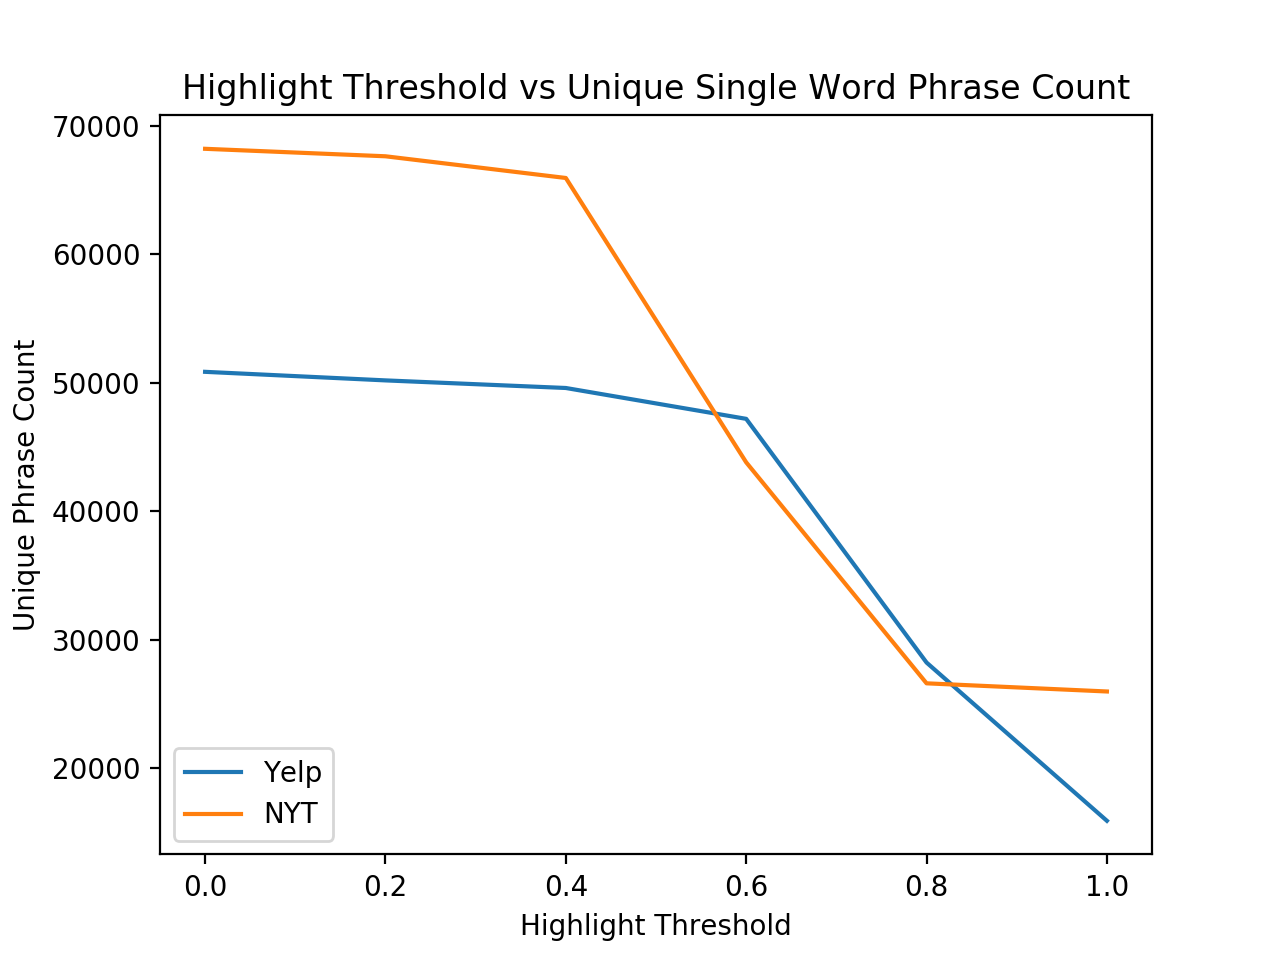
\includegraphics{images/single_word.png}
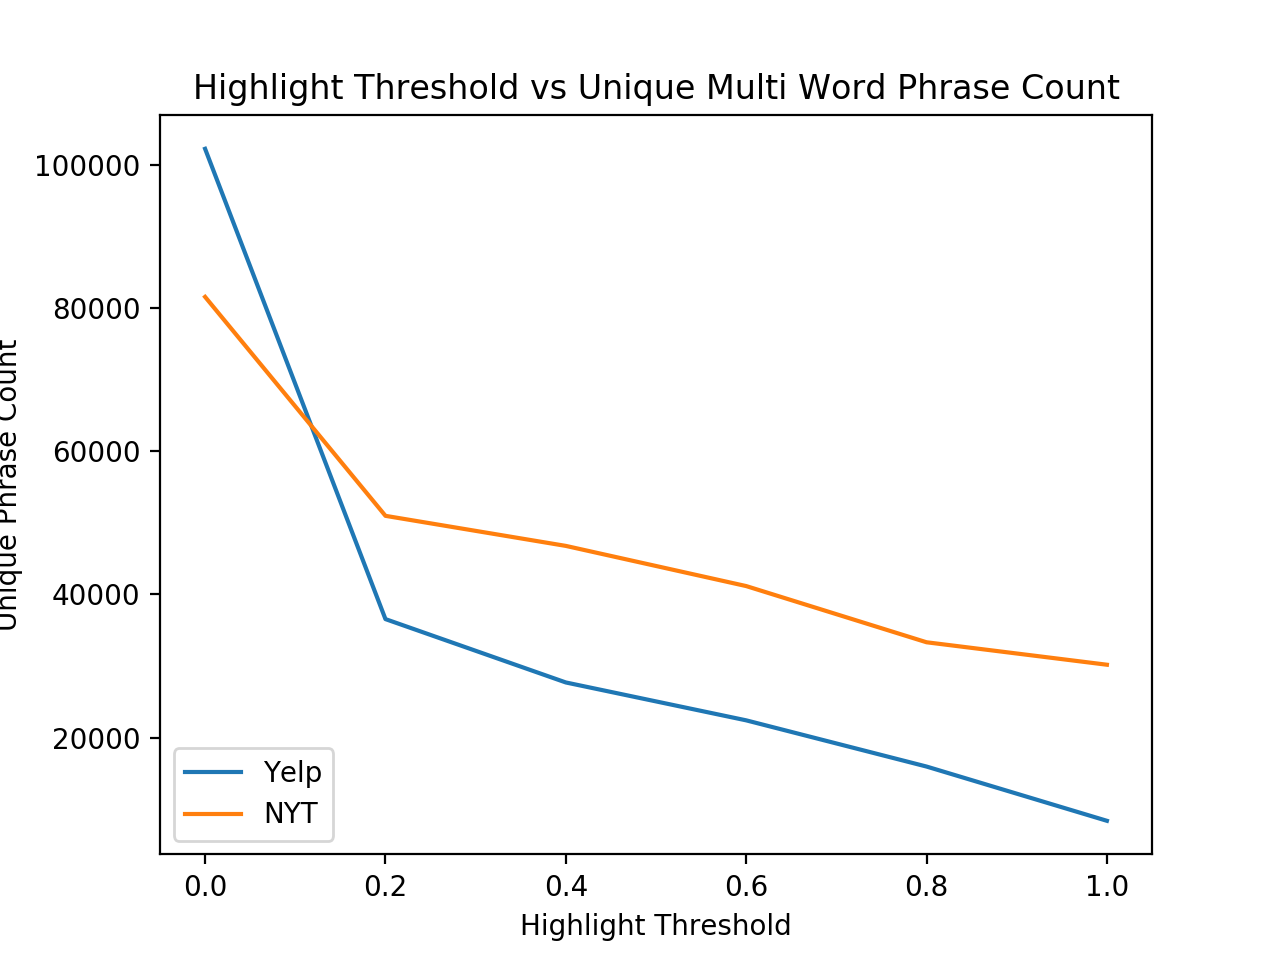
\includegraphics{images/multi_word.png}
\end{figure}
\section*{NYT Clustering Parameters}
Below I will show samples from 3 different clustering results on the NYT dataset.  Each row is from the same clustering iteration and has the same number of centers, the centers are stated in the captions.\\
The first row of tables shows k=5, second row shows k=20, and the third row shows k=40.  You can see the clusters become more coherent as you read through each level.  For example, at k=5 the Justice/Politics cluster mixes police, family and politics while a similar cluster at k=20 (U.S Government/Foreign Entities) provides more closely related phrases related to the U.S and foreign policy. Furthermore, there is a k=40 cluster (U.S Government) that narrows this down to only the U.S.
\begin{table}[ht]
    \parbox{.25\linewidth}{
    \centering
    \begin{tabular}{|c|}
    \hline
    \_government\_\\
    \hline
    \_U.S\_\\
    \hline
    \_state\_\\
    \hline
    \_United\_States\_\\
    \hline
    \_country\_\\
    \hline
    \_long\_\\
    \hline
    \_public\_\\
    \hline
    \_city\_\\
    \hline
    \_American\_\\
    \hline
    \_political\_\\
    \hline
    \end{tabular}
    \caption{k=5: Government/Politics}
    }
    \hfill
    \parbox{.25\linewidth}{
    \centering
    \begin{tabular}{|c|}
    \hline
    \_game\_\\
    \hline
    \_season\_\\
    \hline
    \_play\_\\
    \hline
    \_games\_\\
    \hline
    \_lead\_\\
    \hline
    \_led\_\\
    \hline
    \_lost\_\\
    \hline
    \_shot\_\\
    \hline
    \_free\_\\
    \hline
    \_history\_\\
    \hline
    \end{tabular}
    \caption{k=5: Sports/Games}
    }
    \hfill
    \parbox{.25\linewidth}{
    \centering
    \begin{tabular}{|c|}
    \hline
    \_police\_\\
    \hline
    \_family\_\\
    \hline
    \_law\_\\
    \hline
    \_court\_\\
    \hline
    \_federal\_\\
    \hline
    \_death\_\\
    \hline
    \_party\_\\
    \hline
    \_Republican\_\\
    \hline
    \_South\_\\
    \hline
    \_President\_\\
    \hline
    \end{tabular}
    \caption{k=5: Justice/Politics}
    }
\end{table}\\
\begin{table}[ht]
    \parbox{.25\linewidth}{
    \centering
    \begin{tabular}{|c|}
    \hline
    \_United\_States\_\\
    \hline
    \_president\_\\
    \hline
    \_China\_\\
    \hline
    \_European\_\\
    \hline
    \_President\_\\
    \hline
    \_Iran\_\\
    \hline
    \_Europe\_\\
    \hline
    \_Russia\_\\
    \hline
    \_trade\_\\
    \hline
    \_France\_\\
    \hline
    \end{tabular}
    \caption{k=20: U.S Government/Foreign Entities}
    }
    \hfill
    \parbox{.25\linewidth}{
    \centering
    \begin{tabular}{|c|}
    \hline
    \_city\_\\
    \hline
    \_military\_\\
    \hline
    \_security\_\\
    \hline
    \_French\_\\
    \hline
    \_British\_\\
    \hline
    \_violence\_\\
    \hline
    \_war\_\\
    \hline
    \_corruption\_\\
    \hline
    \_United\_Nations\_\\
    \hline
    \_Afghanistan\_\\
    \hline
    \end{tabular}
    \caption{k=20: Military/War}
    }
    \hfill
    \parbox{.25\linewidth}{
    \centering
    \begin{tabular}{|c|}
    \hline
    \_company\_\\
    \hline
    \_business\_\\
    \hline
    \_director\_\\
    \hline
    \_research\_\\
    \hline
    \_firm\_\\
    \hline
    \_chief\_executive\_\\
    \hline
    \_general\_\\
    \hline
    \_organization\_\\
    \hline
    \_Department\_\\
    \hline
    \_Center\_\\
    \hline
    \end{tabular}
    \caption{k=20: Business}
    }
\end{table}\\
\begin{table}[ht]
    \parbox{.25\linewidth}{
    \centering
    \begin{tabular}{|c|}
    \hline
    \_long\_\\
    \hline
    \_high\_\\
    \hline
    \_fell\_\\
    \hline
    \_average\_\\
    \hline
    \_rose\_\\
    \hline
    \_short\_\\
    \hline
    \_stock\_\\
    \hline
    \_lower\_\\
    \hline
    \_unemployment\_\\
    \hline
    \_reading\_\\
    \hline
    \end{tabular}
    \caption{k=40: Economy/Stocks}
    }
    \hfill
    \parbox{.25\linewidth}{
    \centering
    \begin{tabular}{|c|}
    \hline
    \_Republican\_\\
    \hline
    \_Senate\_\\
    \hline
    \_House\_\\
    \hline
    \_Republicans\_\\
    \hline
    \_Congress\_\\
    \hline
    \_White\_House\_\\
    \hline
    \_Texas\_\\
    \hline
    \_Democrats\_\\
    \hline
    \_Democratic\_\\
    \hline
    \_Democrat\_\\
    \hline
    \end{tabular}
    \caption{k=40: U.S Government}
    }
    \hfill
    \parbox{.25\linewidth}{
    \centering
    \begin{tabular}{|c|}
    \hline
    \_England\_\\
    \hline
    \_captain\_\\
    \hline
    \_Chelsea\_\\
    \hline
    \_New\_Zealand\_\\
    \hline
    \_Premier\_League\_\\
    \hline
    \_Champions\_League\_\\
    \hline
    \_Arsenal\_\\
    \hline
    \_Liverpool\_\\
    \hline
    \_Barcelona\_\\
    \hline
    \_squad\_\\
    \hline
    \end{tabular}
    \caption{k=40: Soccer}
    }
\end{table}\\
\section*{Yelp Clustering Parameters}
Below I will show samples from 3 different clustering results on the Yelp dataset.  Each row is from the same clustering iteration and has the same number of centers, the centers are stated in the captions.\\
The first row of tables shows k=5, second row shows k=20, and the third row shows k=40.  You can see the clusters become more coherent as you read through each level.  For example, at k=5 there is a Miscellaneous cluster in which the phrases don't seem to be related,  while the clusters at k=20 are more conceptually similar. Furthermore, there is a k=40 cluster (Decorations) that is much more specific than any cluster in k=20 or k=5.
\begin{table}[ht]
    \parbox{.25\linewidth}{
    \centering
    \begin{tabular}{|c|}
    \hline
    \_food\_\\
    \hline
    \_restaurant\_\\
    \hline
    \_stars\_\\
    \hline
    \_sushi\_\\
    \hline
    \_happy\_hour\_\\
    \hline
    \_star\_\\
    \hline
    \_Thai\_\\
    \hline
    \_average\_\\
    \hline
    \_Food\_\\
    \hline
    \_Chicken\_\\
    \hline
    \end{tabular}
    \caption{k=5: Restaurants/Food}
    }
    \hfill
    \parbox{.25\linewidth}{
    \centering
    \begin{tabular}{|c|}
    \hline
    \_order\_\\
    \hline
    \_long\_\\
    \hline
    \_free\_\\
    \hline
    \_water\_\\
    \hline
    \_music\_\\
    \hline
    \_car\_\\
    \hline
    \_money\_\\
    \hline
    \_glass\_\\
    \hline
    \_manager\_\\
    \hline
    \_game\_\\
    \hline
    \end{tabular}
    \caption{k=5: Miscellaneous}
    }
    \hfill
    \parbox{.25\linewidth}{
    \centering
    \begin{tabular}{|c|}
    \hline
    \_nice\_\\
    \hline
    \_friendly\_\\
    \hline
    \_bit\_\\
    \hline
    \_atmosphere\_\\
    \hline
    \_high\_\\
    \hline
    \_sat\_\\
    \hline
    \_Love\_\\
    \hline
    \_variety\_\\
    \hline
    \_park\_\\
    \hline
    \_Nice\_\\
    \hline
    \end{tabular}
    \caption{k=5: Descriptions}
    }
\end{table}\\
\begin{table}[ht]
    \parbox{.25\linewidth}{
    \centering
    \begin{tabular}{|c|}
    \hline
    \_food\_\\
    \hline
    \_restaurant\_\\
    \hline
    \_stars\_\\
    \hline
    \_sushi\_\\
    \hline
    \_star\_\\
    \hline
    \_Thai\_\\
    \hline
    \_average\_\\
    \hline
    \_Food\_\\
    \hline
    \_Mexican\_\\
    \hline
    \_Italian\_\\
    \hline
    \end{tabular}
    \caption{k=20: Food Types}
    }
    \hfill
    \parbox{.25\linewidth}{
    \centering
    \begin{tabular}{|c|}
    \hline
    \_sandwich\_\\
    \hline
    \_fries\_\\
    \hline
    \_shrimp\_\\
    \hline
    \_steak\_\\
    \hline
    \_sandwiches\_\\
    \hline
    \_appetizer\_\\
    \hline
    \_salads\_\\
    \hline
    \_pasta\_\\
    \hline
    \_egg\_\\
    \hline
    \_eggs\_\\
    \hline
    \end{tabular}
    \caption{k=20: Food Items}
    }
    \hfill
    \parbox{.25\linewidth}{
    \centering
    \begin{tabular}{|c|}
    \hline
    \_order\_\\
    \hline
    \_friendly\_\\
    \hline
    \_friends\_\\
    \hline
    \_family\_\\
    \hline
    \_sat\_\\
    \hline
    \_manager\_\\
    \hline
    \_party\_\\
    \hline
    \_bartender\_\\
    \hline
    \_talk\_\\
    \hline
    \_chef\_\\
    \hline
    \end{tabular}
    \caption{k=20: Food Service}
    }
\end{table}\\
\begin{table}[ht]
    \parbox{.25\linewidth}{
    \centering
    \begin{tabular}{|c|}
    \hline
    \_friendly\_\\
    \hline
    \_manager\_\\
    \hline
    \_customer\_service\_\\
    \hline
    \_bartender\_\\
    \hline
    \_talk\_\\
    \hline
    \_company\_\\
    \hline
    \_chef\_\\
    \hline
    \_professional\_\\
    \hline
    \_management\_\\
    \hline
    \_super\_friendly\_\\
    \hline
    \end{tabular}
    \caption{k=40: Customer Service}
    }
    \hfill
    \parbox{.25\linewidth}{
    \centering
    \begin{tabular}{|c|}
    \hline
    \_sandwich\_\\
    \hline
    \_fries\_\\
    \hline
    \_bread\_\\
    \hline
    \_steak\_\\
    \hline
    \_sandwiches\_\\
    \hline
    \_bacon\_\\
    \hline
    \_salads\_\\
    \hline
    \_eggs\_\\
    \hline
    \_onion\_\\
    \hline
    \_sausage\_\\
    \hline
    \end{tabular}
    \caption{k=40: Food Items}
    }
    \hfill
    \parbox{.25\linewidth}{
    \centering
    \begin{tabular}{|c|}
    \hline
    \_art\_\\
    \hline
    \_center\_\\
    \hline
    \_brand\_\\
    \hline
    \_dining\_room\_\\
    \hline
    \_furniture\_\\
    \hline
    \_bar\_area\_\\
    \hline
    \_private\_\\
    \hline
    \_stock\_\\
    \hline
    \_bakery\_\\
    \hline
    \_design\_\\
    \hline
    \end{tabular}
    \caption{k=40: Decorations}
    }
\end{table}\\
\end{document}
